
\section{����}
\label{sec4_1}

This section discusses the design of the segmentation pipeline and details the principles of the consisting modules.
Fig. \ref{fig:DataFlow4} presents the block diagram of the processing pipeline in the bird's-eye view.
The data type of the pixels in the original images is firstly converted.
After the images are appropriately thresholded, the data needs to be enhanced appropriately, right before sending the data to the downstream modules.
The enhancement should highlight the ``tube-like" objects, which are the coronary arteries in this paper.
Next the intensities of the enhanced objects are tuned for the following processing.
Then two computations are performed simultaneously to generate the speed images and the initial contours for the CURVES system.
After that, the results are fed into the CURVES module, where the actual fronts propagation occurs.
The CURVES system can evolve the input contours with the reference of the speed images until the contours ``touches" the wall of the tiny vessels.
Finally the output contours are extracted and then visualized in the surface rendering way.
\begin{figure}[t]
\centering
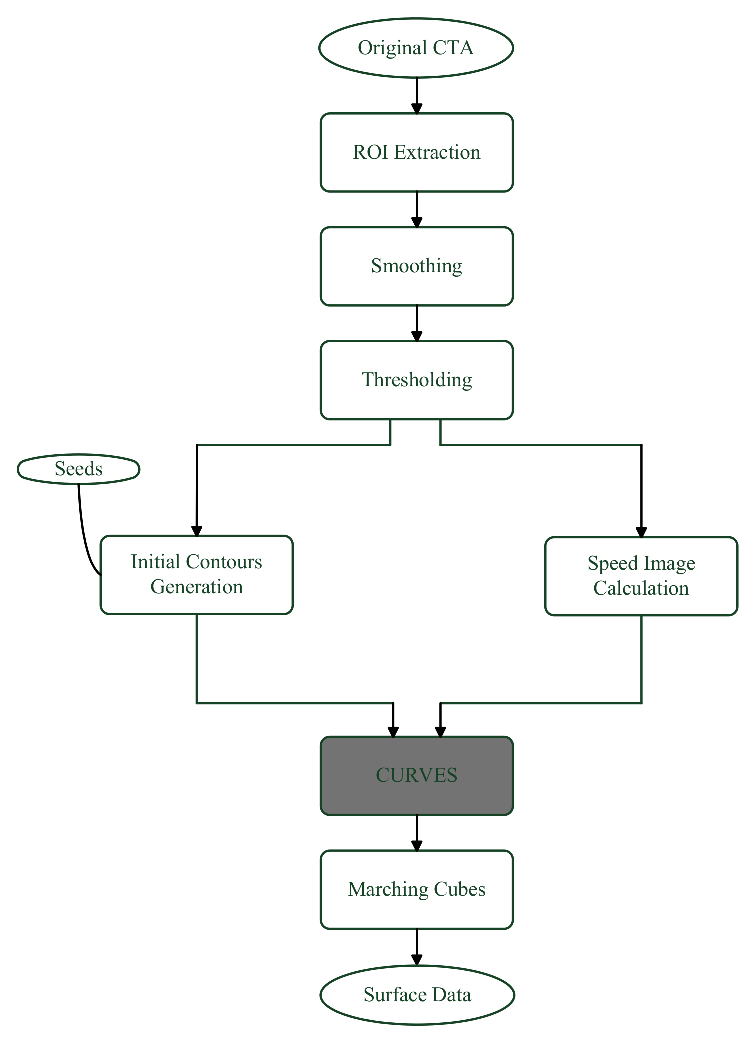
\includegraphics[height=3.2in,width=3.2in]{figures/chap04/DataFlow.eps}
\caption{Collaboration diagram of the segmentation pipeline.}
\label{fig:DataFlow4}
\end{figure}

\subsection{��״�������ǿ}

The tubular enhancement is a sort of multi-scale line filtering, whose scheme can be summarized as the ``tube-like" objects in the image are highlighted whilst the rest are attenuated. %
To achieve this, the three dimensional multi-scale algorithm proposed by Sato \textit{et al.} \cite{Sato1998} is introduced.

To shape the filter response to certain width of lines and suppress the noisy effects, the pixels need to convolving with the second order derivatives of a Gaussian kernel.
This computation is an equivalent to the calculation of the Hessian matrix $\mathcal{H}$ of the three-dimensional image $I(\cdot)$:
\begin{gather}
\label{eqn:Hessian}
\mathcal{H} = \nabla^2 I =
\begin{bmatrix}
I_{xx} & I_{xy} & I_{xz} \\ I_{yx} & I_{yy} & I_{yz} \\ I_{zx} & I_{zy} & I_{zz}
\end{bmatrix},
\end{gather}
where $I_{xx} = \frac{\partial^2 I}{\partial^2 x}$, $I_{xy} = \frac{\partial^2 I}{\partial x \partial y}$, to name a few.
And all these partial second order derivatives are the convolutions with the second order derivatives of a Gaussian kernel $G(x; \sigma)$ with the standard deviation $\sigma$:
\begin{equation}
\label{GaussianConvolution}
I_{xx} = I \ast \frac{\partial^2 G}{\partial^2 x}.
\end{equation}
The eigenvalues of (\ref{eqn:Hessian}) are $\lambda_1$, $\lambda_2$, and $\lambda_3$ with their values in descending order.
Their associated eigenvectors are $e_1$, $e_2$, and $e_3$, respectively.

When $\lambda_1 \approx 0$ and $\lambda_2 \approx \lambda_3 \ll 0$, the line measure can be written as
\begin{equation}
\label{eqn:LineMeasure}
\lambda_{123} =
\begin{cases}
\left| \lambda_3 \right| \left( \frac{\lambda_2}{\lambda_3} \right)^{\gamma_{23}} \left( 1 + \frac{\lambda_1}{\left| \lambda_2 \right|} \right)^{\gamma_{12}}, & \lambda_1 \le 0 \\
\left| \lambda_3 \right| \left( \frac{\lambda_2}{\lambda_3} \right)^{\gamma_{23}} \left( 1 - \alpha \frac{\lambda_1}{\left| \lambda_2 \right|} \right)^{\gamma_{12}}, & \frac{\left| \lambda_2 \right|}{\alpha} > \lambda_1 > 0 \\
0, & \text{otherwise}.
\end{cases}
\end{equation}
In (\ref{eqn:LineMeasure}), the additional parameters $\gamma_{12}$, $\gamma_{23}$, and $\alpha$ are all positive constant, where $\gamma_{12} \in [0, \infty)$ is used to discriminate between the branching structures and the noises as well as pseudo-branches, $\gamma_{23} \in [0, \infty)$ regulates the sharpness, and $\alpha \in (0, 1.0]$ maintains the asymmetrical characteristics of the last terms of the function for all possible $\lambda_1$.

Additionally, different choices of the eigenvalues can equip the line filter with the abilities in detecting different shapes of the objects as shown in Table. \ref{tbl:Eigenvalues}. %

\subsection{ˮƽ���ݽ�֮ǰ��Ԥ����}

\subsubsection{����ͼ��ļ���}

Level set algorithms evolves the contours in the gradient field with ``sharp" variations in intensity values from the inner or outer area to the boundaries.
The aim of the speed images is to provide this gradient field in the form of nicely shaped gradient images.
In the gradient images, the magnitude of the gradient at each pixel is calculated.
Next the gradient images $I_{\nabla}$ are transformed into the speed images $I_{\sigma}$ by applying the nonlinear relation:
\begin{equation}
\label{eqn:Sigmoid}
I_{\sigma} = (I_{max} - I_{min}) \cdot \frac{1}{1 + \exp\left(-\frac{I_{\nabla} - n}{m}\right)} + I_{min},
\end{equation}
where $I_{max}$ and $I_{min}$ are the two extreme values of the output intensity values, $m$ is a constant that controls the window width of the input intensity, and $n$ is a constant that defines the center of the window.
\begin{table}
\renewcommand{\arraystretch}{1.3}
\caption{Eigenvalue sets for detecting different shapes}
\label{tbl:Eigenvalues}
\centering
\begin{tabular}{l||c}
\hline
\bfseries Shape & \bfseries Eigenvalues \\
\hline\hline
Bright tubes   & $\lambda_1 \approx 0, \lambda_2 \approx \lambda_3 \ll 0$ \\
Dark tubes     & $\lambda_1 \approx 0, \lambda_2 \approx \lambda_3 \gg 0$ \\
Bright plates  & $\lambda_1 \approx \lambda_2 \approx 0, \lambda_3 \ll 0$ \\
Dark plates    & $\lambda_1 \approx \lambda_2 \approx 0, \lambda_3 \gg 0$ \\
Bright spheres & $\lambda_1 \approx \lambda_2 \approx \lambda_3 \ll 0$ \\
Dark spheres   & $\lambda_1 \approx \lambda_2 \approx \lambda_3 \gg 0$ \\
\hline
\end{tabular}
\end{table}

\subsubsection{һ�ָĽ���Fast Marching����}

The aim of the colliding fronts module is to evolve the contours for the CURVES system from the user-defined seeding points.
The colliding fronts method is implemented based on the principles of the fast marching algorithm \cite{Sethian1999}.
However, this method requires two seeds for each round of evolution such that the area between the seeds can be extracted.
The output of this module is the dot production of the gradient field of arrival times of the two wavefronts.
The level set initialization for the prolonged objects greatly benefit from this feature of the method.
On the other hand, the method also shortens the computation time.

\subsection{CURVES�ݽ�ģ��}

The CURVES method \cite{Lorigo2001} is chosen as the functioning segmentation method because of the complex nature of the coronary arteries.
It is highly effective in the segmentation of the complicated curvilinear structures in the volumetric medical images.
In addition, the criterion of CURVES method also takes the local smoothness of the boundaries to be detected (i.e., the inner wall of the coronary arteries) into account.

This method is a modification of the geodesic active contours method developed in Caselles \textit{et al.} \cite{Caselles1997}.
As the extensive research of the geodesic active contours, CURVES is a level set algorithm that models the tiny vessels as spatial curves with arbitrarily complicated topology \cite{Lorigo2001}. %
CURVES evolves the level sets to the boundaries of the targets based on the criterion of the minimization of the following energy functional
\begin{equation}
\label{eqn:CURVES}
\oint_0^1 g\left( \left| \nabla I \left( \mathcal{C} \left(  s \right) \right) \right| \right) \left| \mathcal{C}'\left( s \right) \right| ds,
\end{equation}
where $\mathcal{C}\left( s \right): [0,1] \rightarrow \mathrm{R}^3$ is a one-dimension curve, $I\left( \cdot \right): [0, a] \times [0, b] \times [0, c] \rightarrow [0, \infty)$ is an image on which the curve evolution takes place, and $g\left( \cdot \right): [0, \infty) \rightarrow \mathrm{R}^+$ is a monotonically decreasing function. %

The minimization of this functional can be achieved by searching for the gradient descent direction of the functional itself, which means the Euler-Lagrange equations associated with (\ref{eqn:CURVES}) needs to be computed. %
Thus the geodesic flow equation that controls the contour evolution in this process of minimization can be obtained as follows
\begin{equation}
\label{eqn:Evolution}
\frac{\partial \mathcal{C}}{\partial t} = k \mathcal{N} - \frac{g'}{g} \varPi \left( \mathcal{H} \frac{\nabla I}{ \left| \nabla I \right| } \right),
\end{equation}
where $\mathcal{H}$ is the Hessian matrix of the image $I$, $k$ is the Euclidean curvature, $\mathcal{N}$ is the unit normal vector, $\varPi(\cdot)$ is the projection operator projects the argument onto the normal space. %
The update equation can be obtained as
\begin{equation}
\label{eqn:Update}
\frac{\partial v}{\partial t} = \mathcal{F} \left( \nabla v(x, t), \nabla^2 v(x, t) \right) + \frac{g'}{g} \nabla v(x, t) \mathcal{H} \frac{\nabla I}{ \left| \nabla I \right| },
\end{equation}
where $v(\cdot): \mathrm{R}^3 \rightarrow [0, \infty)$ is the embedding function of the curve $\mathcal{C}$, $\mathcal{F} \left( \nabla v(x, t), \nabla^2 v(x, t) \right)$ is the smaller eigenvalue of the matrix $P_{\nabla v} \nabla^2 v P_{\nabla v}$. %
The matrix $P_q$ is defined as a projector which projects some vector onto the normal plane of vector $q \in \mathrm{R}^3$:
\begin{equation}
\label{eqn:ProjectionOperator}
P_q = I_0 - \frac{qq^T}{\left| q \right|^2},
\end{equation}
where $I_0$ denotes the identity matrix.

By incorporating the speed images $I_{\sigma}$ to the evolution equation (\ref{eqn:Evolution}), the evolution in our case can be obtained as
\begin{equation}
\label{eqn:Application}
\frac{\partial \mathcal{C}}{\partial t} = k \mathcal{N} - \frac{g'(I_{\sigma})}{g(I_{\sigma})} \varPi \left( \mathcal{H} \frac{\nabla I_{\sigma}}{ \left| \nabla I_{\sigma} \right| } \right).%
\end{equation}

\subsection{��ֵ����Ⱦ}

The surface information is extracted for the visualization by the marching cubes method \cite{Lorensen1987MC}.
Cubes are created based on the input information and are organized into an array structure.
Each cube consists of eight pixels (each four pixels are from a slice).
The index of each cube is labeled by comparing the intensity values of every pixel to the isovalue of the surfaces.
Next the patterns of the intersection between objects and cubes are initially determined based on the triangulated cases.
Then the precise intersection are computed using linear interpolation with the intensity values at each vertex.
The unit normals to the surface are calculated via central differences for the vertices of the cubes.
Finally the generated triangles are ready for the surface rendering. 